%%%%%%%%%%%%%%%%%%%%%%%%%%%%%%%%%%%%%%%%%%%%%%%%%%%%%%%%%%%%%%%%%%%%%%%%%%%%%%%%

% IEEEconf.cls file must exist in the same directory as the TeX file you want to compile
\documentclass[letterpaper, 10 pt, conference]{IEEEconf}

\title{\LARGE \bf
Homework 2:\The Dream Computer
}

\author{Jordan Medina\Kenji Helms\Guillmer Germino
\small 900354172\
\small jordan.medina@student.nmt.edu\
\small {September 18, 2020}
}

% Image/graphics support
\usepackage{graphicx} % takes care of graphic
\graphicspath{ {./images/} } %full file path to the images

% Formatting for lists
\usepackage{enumitem}

% Formatting for media
\usepackage{float}
\restylefloat{table}
\restylefloat{figure}
\usepackage[utf8]{inputenc}
\usepackage{epigraph}


\begin{document}


\maketitle




%%%%%%%%%%%%%%%%%%%%%%%%%%%%%%%%%%%%%%%%%%%%%%%%%%%%%%%%%%%%%%%%%%%%%%%%%%%%%%%%
\section{\underline{Introduction}\ The Confluence of Hardware and Software}

This document is a basic template for writing conference-style                  
reports in LaTeX. You will use this template when writing                       
your report; you will need to replace all text (excluding                       
section headers or preamble information) with the content                       
of your report.

\subsection{Experience}

\epigraph{\textit{Hey, I can dream can't I?}}{Mr. Potato Head \ Toy Story}
I would like to disclose the fact that I have never never built a PC from scratch, taken one apart to study the guts, nor learned the introductory facts necessary to broach the shoreline of this vast ocean of a topic. The closest I can say to having any experience is shopping for a gaming laptop, traversing the lists of components, selecting the beefiest items, and burning fistfulls of cash. All this means is I have a vague idea of manufacturers, and some of their more famous components. Thankfully, this is the Dream Computer, and I will be doing more or less the same thing, and hey, I can dream, can't I?

\section{MY DREAM COMPUTER}

You should list the specification of the computer here. If
you want make a table here, please label the table. See Table
\ref{tbl:example} for an example of a table.

\begin{center}
\begin{tabular}{||c | c | c | c||} 
\hline
  & Product & Price (USD) \ [0.5ex]
\hline\hline
Case & Lian Li Train- 300W Power Supply& $399.95 \ 
\hline
GPU & NVIDIA GEFORCE RTX 3080 & $699.99 \
\hline
CPU & Intel i9-10900 & 439.99 \
\hline
RAM & CORSAIR 32GB2x16GB DDR4 & $126.99 \
\hline
Monitor & Acer Predator X27 & $1999.99 \
\hline
HDD & Toshiba X300 & $115.33\
\hline

\end{tabular}
\caption{Dream Computer Components with Price}
\label{tbl:example}
\end{center}
\end{table}

%%%%%%%%

\subsection{Case}
What is life without a little bit of hilarity? Although I want my high performing components to be housed by something that isn't merely a futuristic light show beneath my desk. The LIAN LI PC-CK101L Black Aluminum Mini-ITX Tower is a beast in its own right, and would be perfect for sprucing up the shiny intensity of the components, with a nod to old school coolness.


\centering
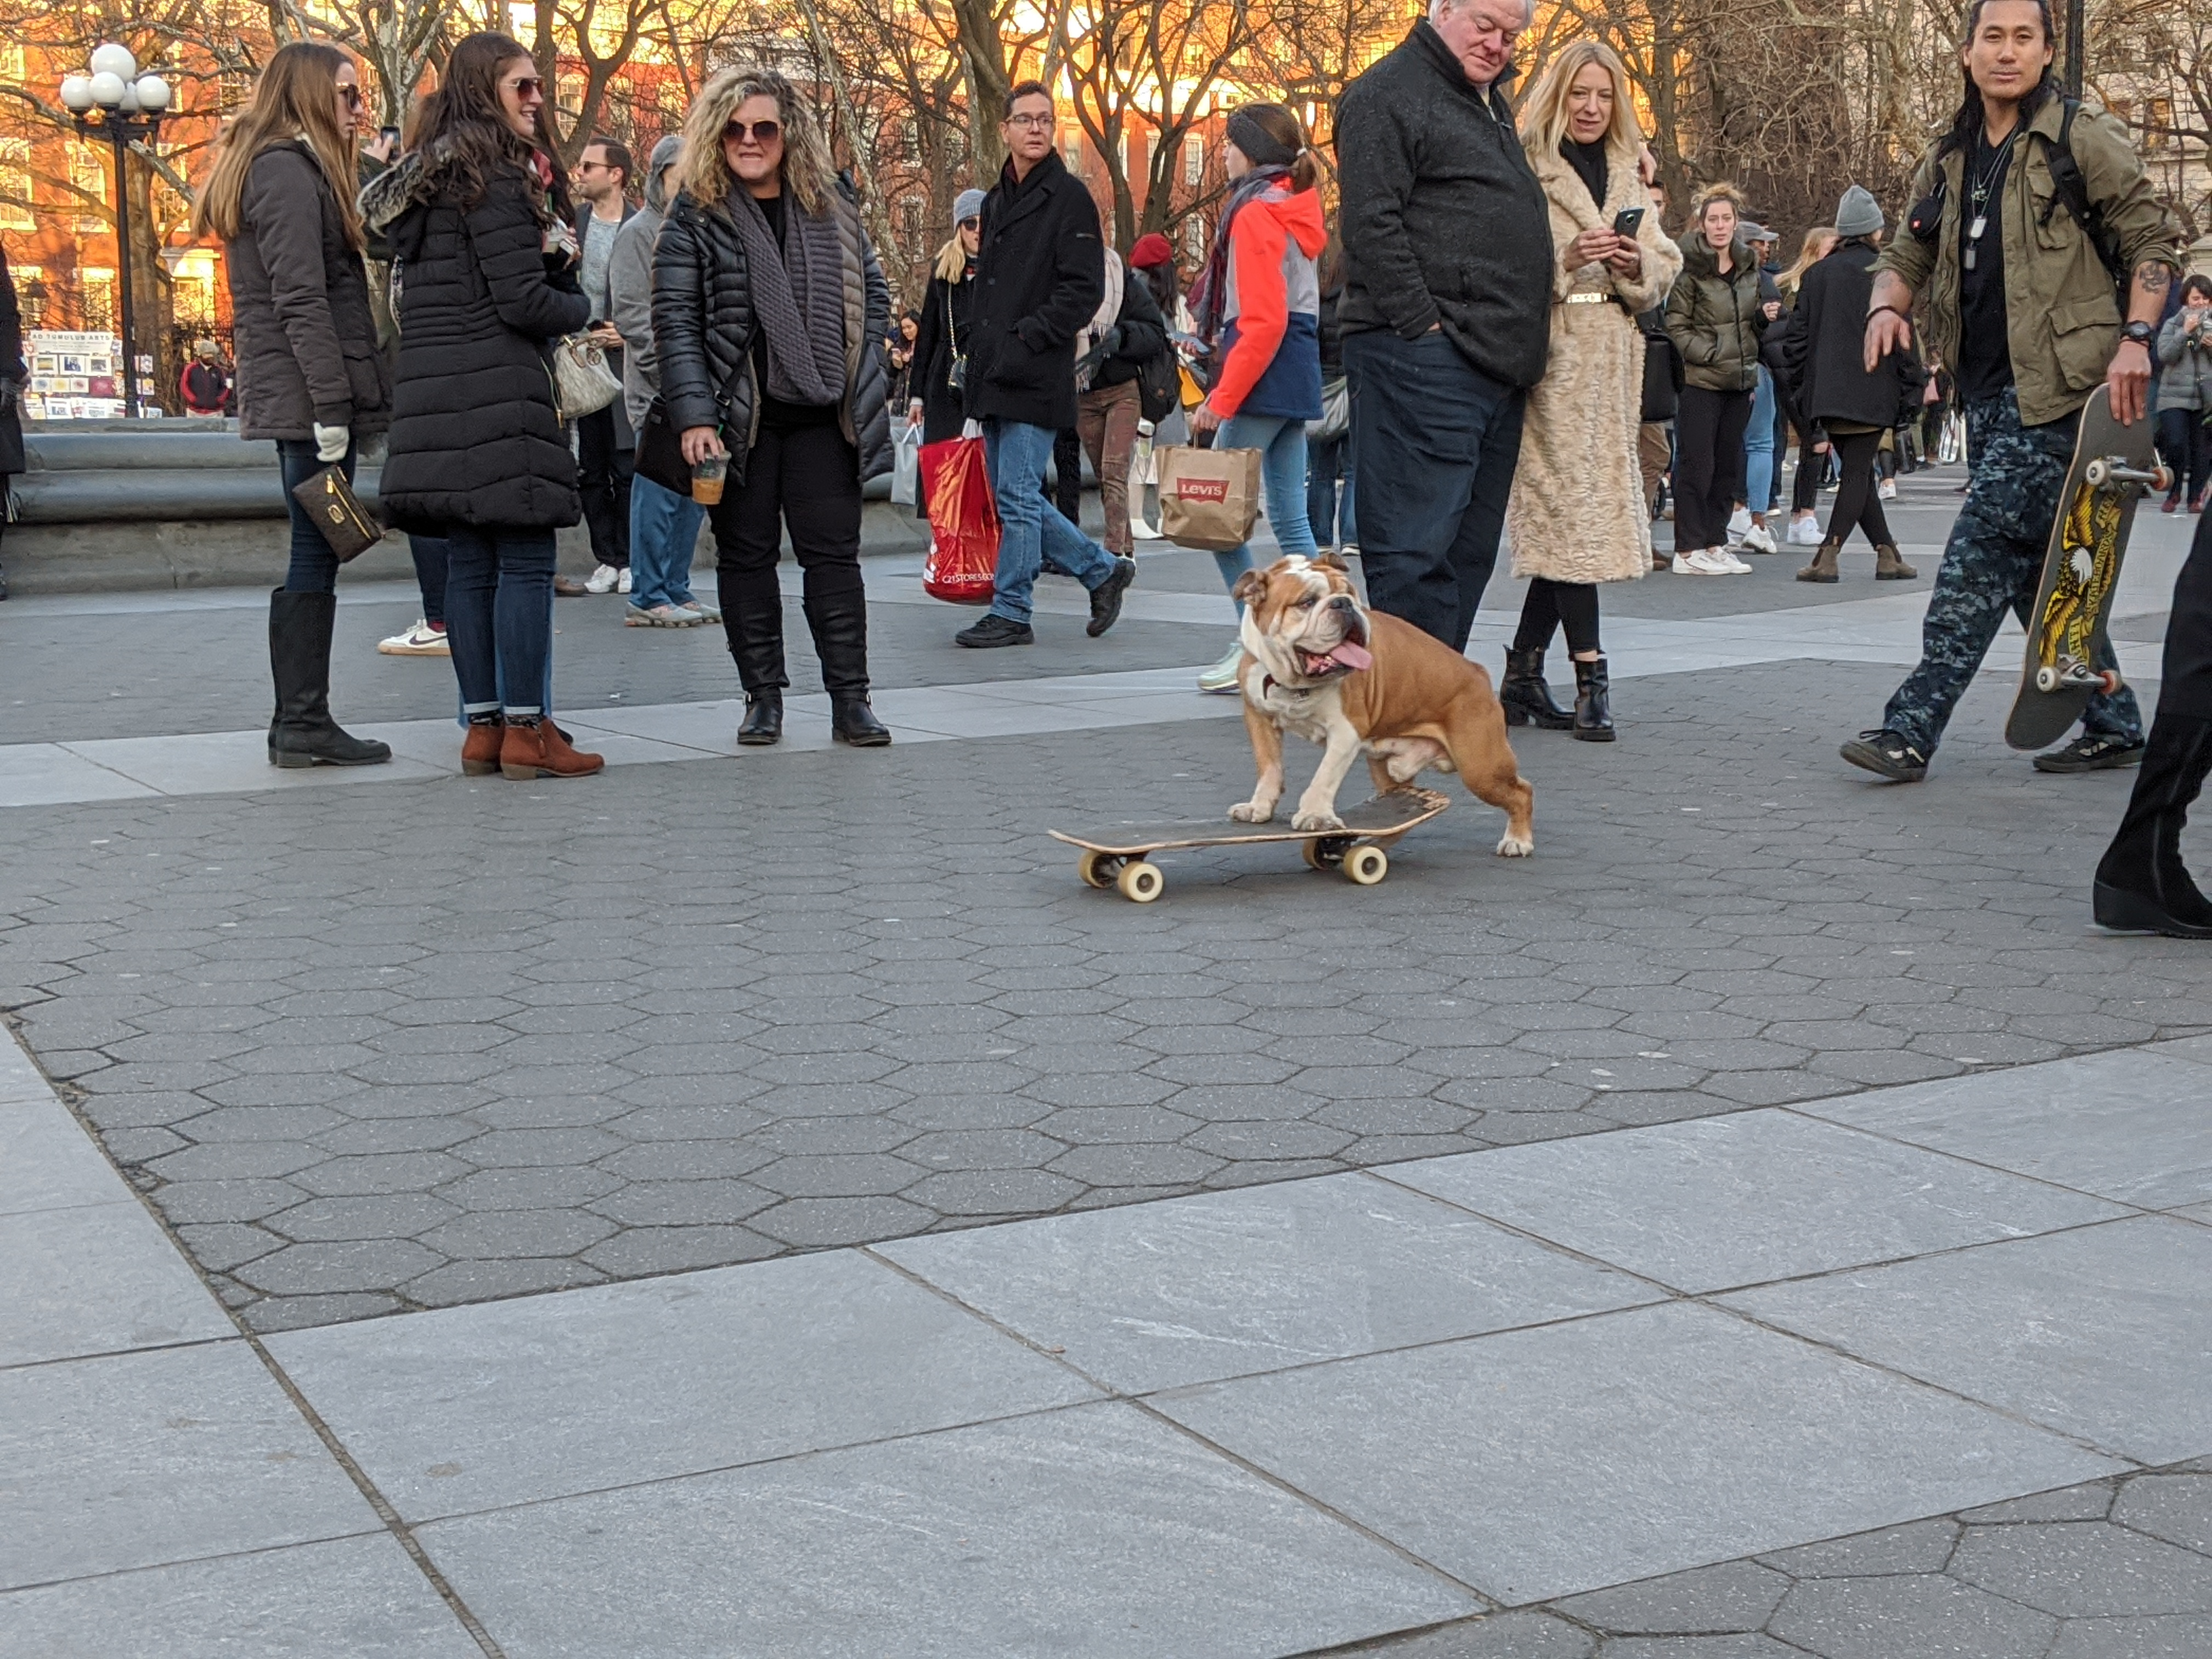
\includegraphics[width=0.2\textwidth]{IMG_20200222_170137.jpg}
\caption{LIAN LI PC-CK101L Black Aluminum Mini-ITX Tower Computer Case 300W Power Supply }
\label{fig:example}
\end{figure} 


\subsection{GPU}

This graphics card will need no introduction, because even an unitiated  member of the NMT CSE Discord server, like myself, will have been rocked by the wake of new NVIDIA-card discussions among the tech-savvy PC builders. I have been a happy owner of a RTX 2080 in my current PC, so I can only lick my lips  thinking about what is possible with NVIDIA's new RTX 3080. I will safely assume all of my gaming needs will be met with this card.
\subsection{CPU}

My CPU was chosen almost exclusively for its age. My current Intel 8th gen Core i9 is doing a fine job, and still isn't required by the modern games I've come across, so I can't the 10th generation will be made obsolete any time soon.
\subsection{Memory}
Although I didn't go as ballistic as possible with the RAM choice, I did choose a sufficiently large enough memory to allow for any of my personal tasks to be accomplished while even running a high end video game. Overclocking with modern RAM will be more than enough to give just enough oomph for anything this humble gamer can muster.
\subsection{Monitor}
When it comes to monitors or TV screens, I really do find myself having an annoying eye to detail. Until my eyeballs melt from the exposure of what our glowing rectangles mete out, I will be pursuing the absolute best quality images that I can buy. The Acer Predator X27 screen is a top class monitor, and looks beautiful. I love HD playback with movies and streaming, and I am in love with what new generations of video games are able to bring to modern 4k screens. This is an indulgence I couldn't possibly regret.

\centering
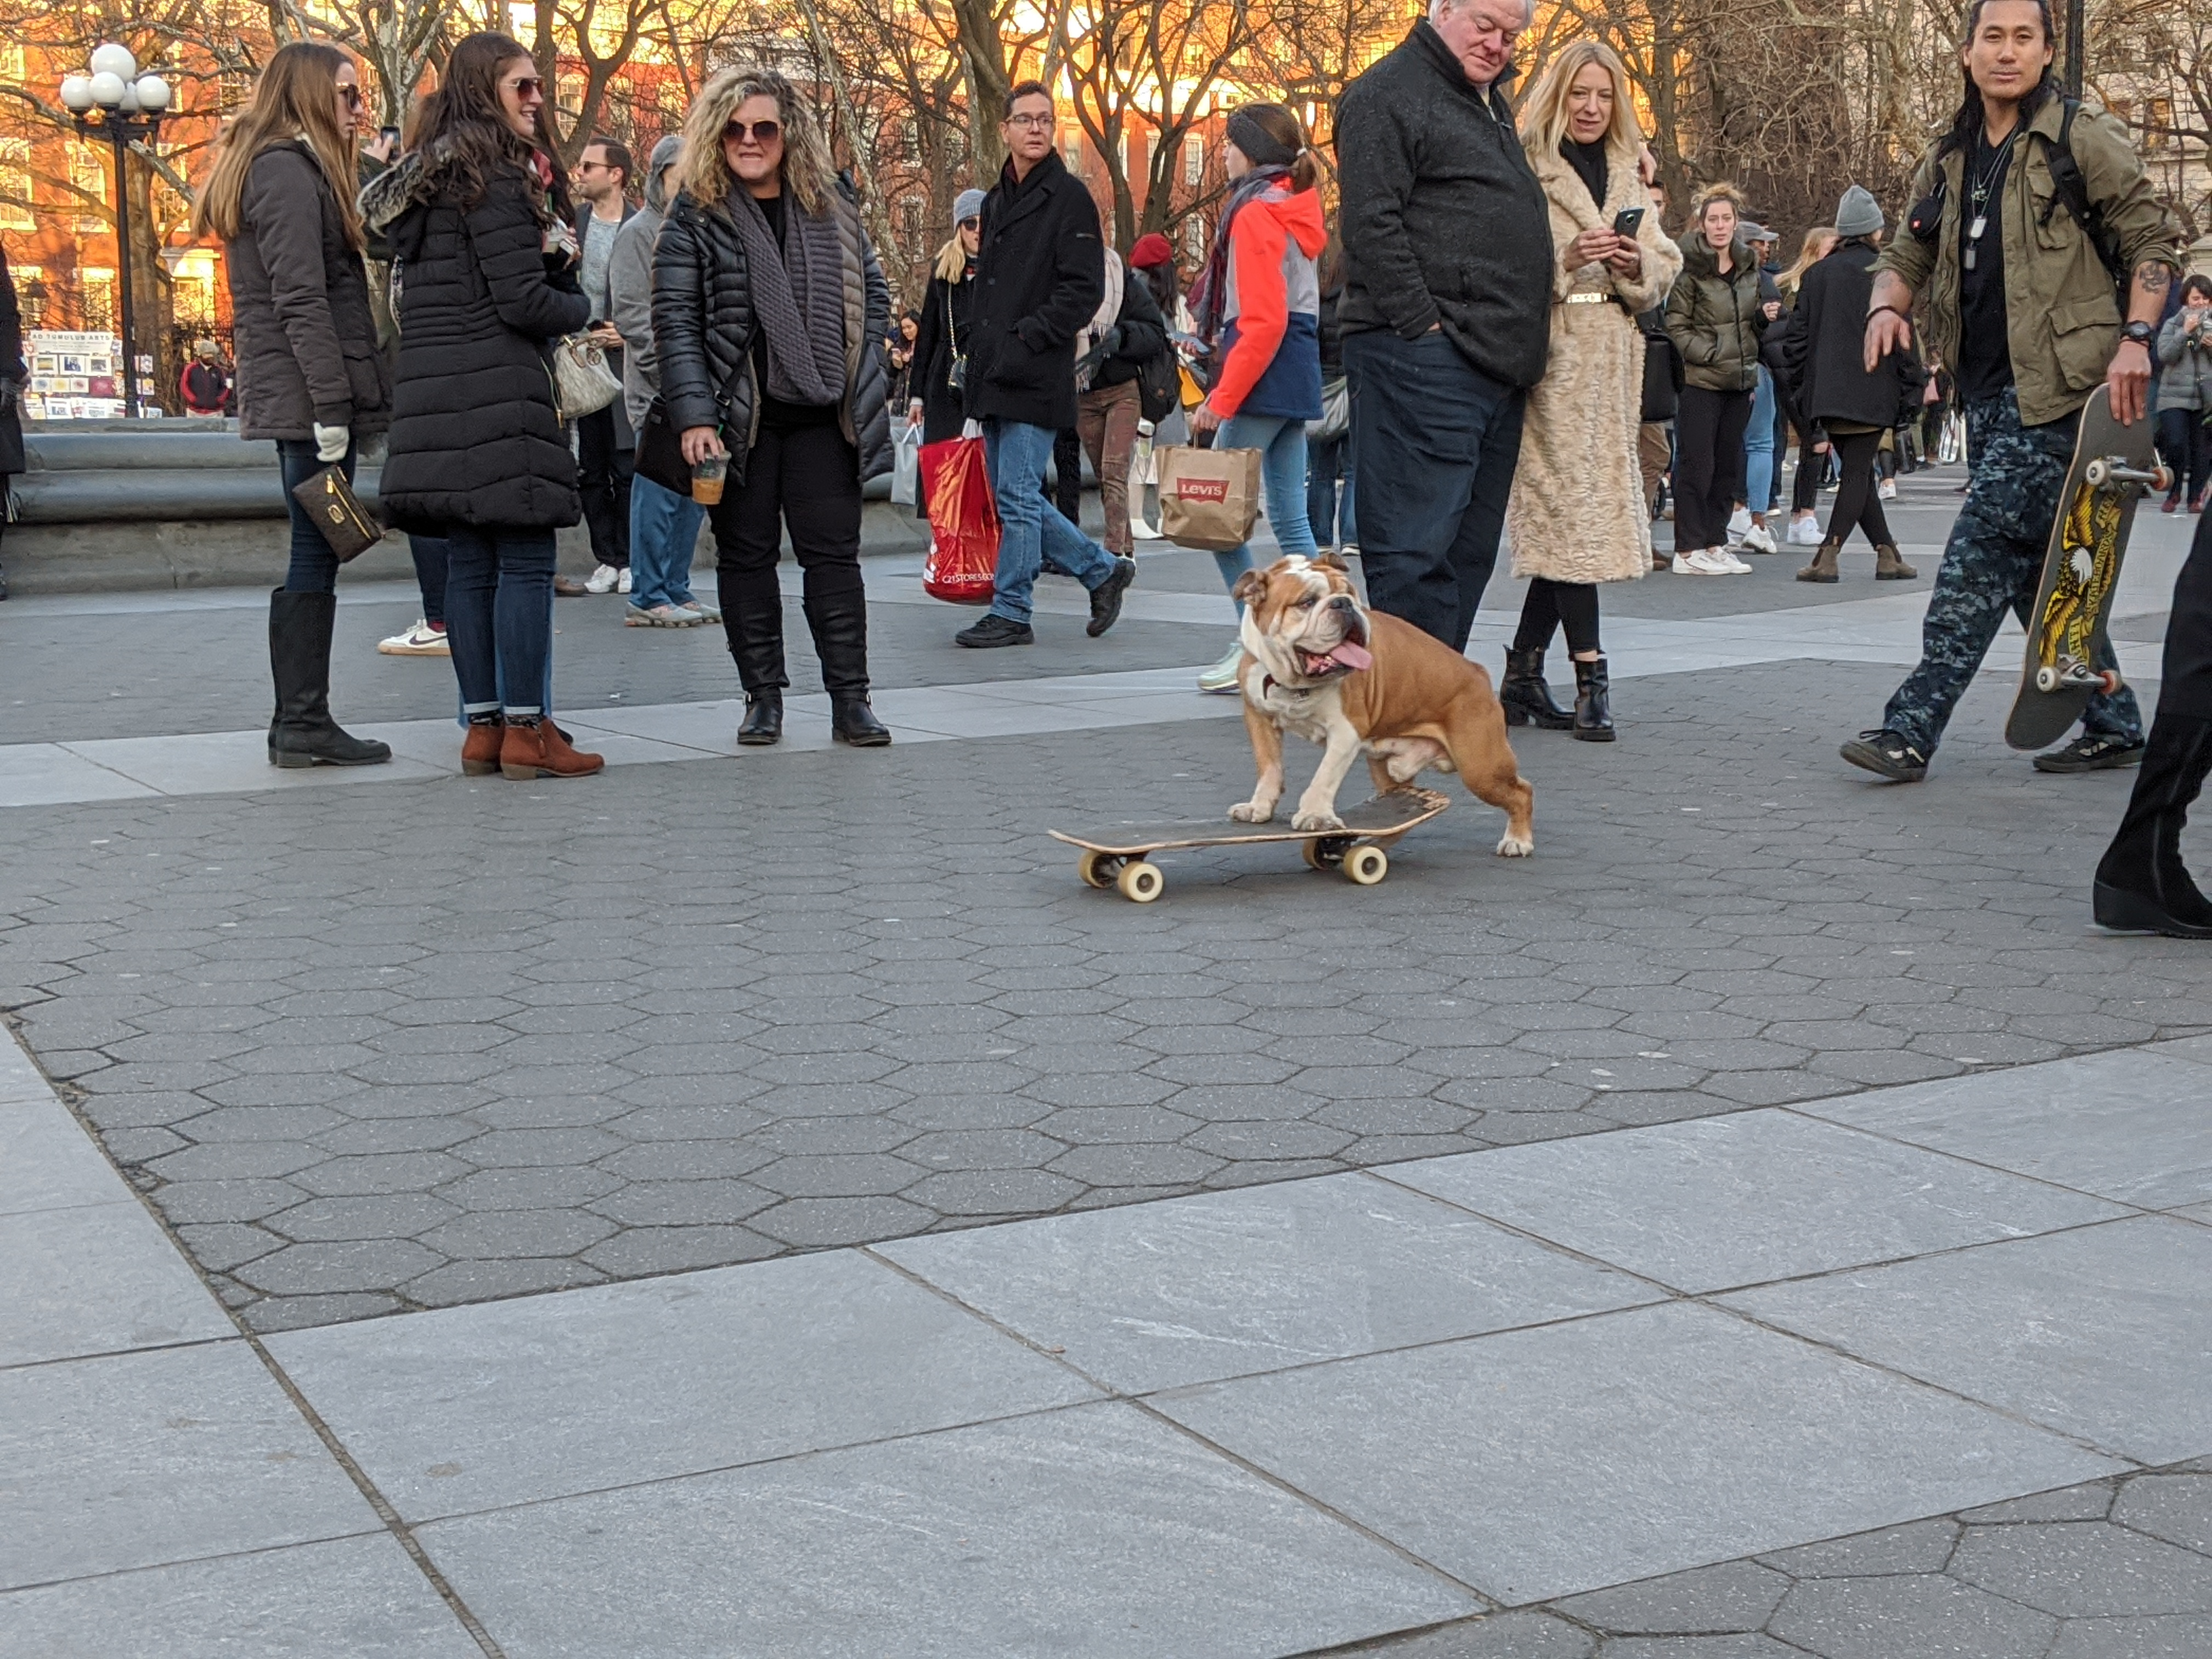
\includegraphics[width=0.2\textwidth]{IMG_20200222_170137.jpg}
\caption{Acer Predator X27 Monitor... oh my}
\label{fig:example}
\end{figure} 

\subsection{HDD}
In this component, size is my only consideration. I do not have enough understanding of alternatives to HDD components, other than their storage space. Here, above all else, is where I know I am exposed as a simple man. As referenced in my introduction, I really just want to know that I'll never have to worry about running out of a particular item's ability. 5TB sounds too much? Yes, yes it does.
\subsection{Total Cost}
With no regard for the cost, I can safely crunch the numbers of my Dream Computer without risk of heart attack:\$399.95 + $699.99 + $439.99 + $126.99+ $1999.99 + $115.33 = \underline{\textbf{$3,782.24}}
\\\footnotesize{I am embarrassed to say that this price is nearly identical to what I have paid for my current Alienware m17 gaming laptop...}

\section{PROBLEMS WITH BUILDING THIS COMPUTER}
Technical know-how is my greatest obstacle for creating this Dream. I realize that I must have skipped out on so many smaller detail parts in this process as well. This is a HUGE problem. A realistic scenario would involve hiring a very trustworthy expert to assemble the pieces I bring them, which would in turn create a labor cost. I would also have to completely rebudget my current living expenses as I pursue my CS degree at NMT, which is the most serious logistic problem, assuming I could reliably build this Dream PC.

\section{CONCLUSION}

Without having the technical expertise necessary to undertake such a large project, I do believe that the components of my Dream Computer are beyond sufficient for my usually ordinary PC gaming routines. I have yet to push the boundaries of my current computer, and I doubt I'd be able to punish a system that is much stronger. Although my budget, parts, and philosophy are not humble in this project, my gaming needs are. The Dream Computer would do just fine for me.

\section*{REFERENCES}


\begin{enumerate}[label={[\arabic*]}]
\item https://www.newegg.com/p/N82E16811112392
\item https://www.nvidia.com/en-us/geforce/graphics-cards/30-series/rtx-3080/
\item https://www.intel.com/content/www/us/en/products/processors/core/i9-processors/i9-10900.html
\item https://www.newegg.com/corsair-32gb-260-pin-ddr4-so-dimm/p/N82E16820236682
\item https://www.pcmag.com/reviews/acer-predator-x27
\item https://www.amazon.com/Toshiba-Performance-Desktop-Internal-HDWE150XZSTA/dp/B013JPLKQK
\end{enumerate}

\end{document}


